\section*{HBase FreqIndexBuilder}

\TODO{Hyungro: fix exercise and replace project where appropriate.}

Write an HBase FreqIndexBuilder program to build an inverted index table which
has the unique term's occurrences in all documents from the clueWeb09 dataset.
Each row record of columnfamily ``frequencies'' is unique, where the rowkey is
the unique term stored in byte format, column name is the documentId that
contains this term, and value is the term frequency shown per document. Note
that each row has multiple columns. The result must be loaded to HBase
clueWeb09IndexTable. Figure 1 shows the schema of clueWeb09IndexTable.

\begin{figure}[!htbp]
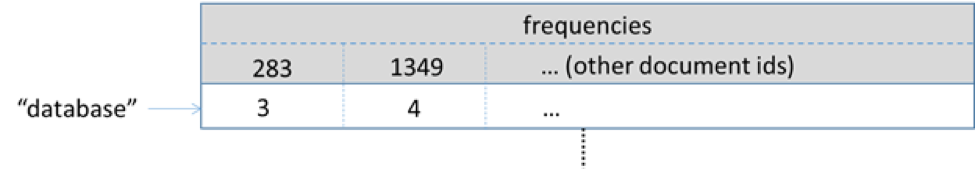
\includegraphics[width=8cm,height=1.5cm]{section/icloud/assignment/exercise5/p5-1}
\centering
\caption{clueWeb09IndexTable table schema for storing term frequencies and their related documentId}
\end{figure}

\subsection*{Deliverables}
Zip your source code, results and report in a file named
username\_exercise5.zip. Submit this file to the Canvas submission page.

\begin{itemize}
\item Complete source code
\item A written report describing the main steps
\end{itemize}

\subsection*{Evaluation}
The point total for this exercise is 3, where the distribution is as follows:
\begin{itemize}
\item Completeness of your code and output (2 points)
\item Correctness of written report (1 points)
\end{itemize}

\subsection*{Introduction}
HBase FreqIndexBuilder is an advanced WordCount program which counts the number
of occurrences of each word in a given text input dataset and also stores the
related document name (identification number) as HBase inverted index records.
These Inverted indices for text data are built for supporting efficient
searches in a huge set of text data.

\subsection*{What is Inverted Index?}
Figure 2 shows an example of an inverted index. For a given set of documents,
each composed of a series of terms (words), it records the following
information: for each term, which subset of documents contains it in their
texts.

To build these inverted indices, we reuse the ClueWeb09 dataset from before,
which was created to support research on information retrieval and related
human language technologies. The dataset is used by several tracks of the TREC
conference. New inverted index table schemas are designed as shown in Figure 1.

In the clueWeb09IndexTable table each term will have the same structure, with
term as rowkey, values contained in documentId, and the occurrence of the term
within this document shown. Our goal is to write an HBase program which
generates an inverted index table by extracting the information from the
ClueWeb09 dataset.

\begin{figure}[!htbp]
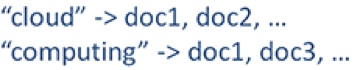
\includegraphics[width=5cm,height=1cm]{section/icloud/assignment/exercise5/p5-2}
\centering
\caption{A sample inverted index}
\end{figure}

\subsection*{Mapper and Main Program}
Now we are going to implement the HBase FreqIndexBuilder program. As opposed to
WordCount, our implementation only consists of two main parts:

\begin{itemize}
\item Mapper
\item Main program
\end{itemize}
This type of application is called ?Map-Only? parallel application.

\subsubsection*{Mapper}
A Mapper overrides the ``map'' function from the Class ``org.apache.hadoop.hbase.mapreduce.TableMapper\\
\textless Text, LongWritable\textgreater'', which provides \textless key, value\textgreater pairs as the input. A Mapper implementation may output \textless key,value\textgreater pairs using the provided Context.
\textless key, value\textgreater of this map function is \textless rowkey, content\textgreater, where the key is the rowkey of an HBase record related to a specified URI, and the content is the stored text of that URI. Your Map task should output \textless word, \textless docId, frequency\textgreater\textgreater for each word in the content of text.

\subsubsection*{Pseudocode}
\begin{lstlisting}[language=Java]
void Map(key, value) {
    for each word x in the content of a hbase record:
    context.write(x, );
}
\end{lstlisting}

\subsubsection*{Detailed implementation}
\lstinputlisting[language=Java]{section/icloud/assignment/exercise5/FibMapper.java}

\subsection*{Main Program}
Again, the main function has been provided as standard initialization, and you
may modify it to fit your own style. See the examples of using
TableMapReduceUtil.initTableMapperJob and
TableMapReduceUtil.initTableReducerJob.

\subsection*{Edit, compile and run your code}
The sketch code is stored within the provided VirtualBox image. You can use
linux text editor vi/vim to add your code.

\begin{lstlisting}[language=bash]
$ cd /root/MoocHomeworks/HBaseInvertedIndexing/
$ vim src/iu/pti/hbaseapp/clueweb09/FreqIndexBuilderClueWeb09.java
$ cd /root/MoocHomeworks/HBaseInvertedIndexing/
$ ./compileAndExecFreqIndexBuilderClueWeb.sh
\end{lstlisting}

\section*{View the result}
The result is generated as /root/hbaseMoocAntProject/output/project2.txt. 
\begin{lstlisting}[language=bash]
$ cd /root/MoocHomeworks/HBaseInvertedIndexing/
$ cat output/project2.txt
\end{lstlisting}

